\section{Optimisation}
\subsection{Cache}
Le cache est une zone de stockage dans laquelle une quantité d'information peut être sauvegardée afin de la rendre accessible et reutilisable très rapidement. En d'autres termes, elle nous permet de réutiliser efficacement les informations qui ont été préalablement stockées.
Pour améliorer le temps de latence de l'application, deux type de caching ont été mis en place.

\subsection{Caching Backend}
Le caching backend a été implementé avec l'aide de Redis. Avant toute chose, il est nécessaire de comprendre ce qu'est Redis.
\begin{figure}[H]
    \begin{minipage}{.3\textwidth}
      
\includegraphics[width=1\linewidth]{img/redis.png}
    \end{minipage}
    \begin{minipage}{.7\textwidth}
Redis est une base de données NoSQL mais elle n'est pas très similaire aux autres bases de données NoSQL. Cela est dû au fait que Redis ne fonctionne pas vraiment avec des tables, mais toutes les données dans Redis sont stockées dans des paires clé-valeur. 
Il y a donc une clé ayant un nom et une valeur appelée Kyle.
L'objectif n'est donc pas de stocker un ensemble de données structurées, mais simplement de stocker une paire clé-valeur individuelle à partir de laquelle nous pouvons accéder aux données.
Il est important de noter que Redis fonctionne en utilisant la mémoire RAM de la machine sur laquelle il tourne, cela signifie qu'il est extrêmement rapide.
\newpara
Dans le cas où nous devons accéder à des informations qui prennent beaucoup de temps à charger, par exemple une quantité de données assez importante provenant de la base de données, nous pouvons utiliser Redis pour stocker ces valeurs pendant une durée définie. Ainsi, lorsque nous devrons accéder à cette même information, la réponse sera beaucoup plus rapide puisque l'information sera déjà chargée.
\end{minipage}
\end{figure}
\subsubsection{Analyse des résultats}
Le temps de chargement des données sur certaines de mes endpoints était assez important et je devais trouver une solution pour le réduire. 
Afin d'améliorer le temps de chargement des données, j'ai décidé d'utiliser Redis. 
Pour tester Redis, j'ai décidé de récuperer tous les clients se trouvant dans ma base de données, ce qui correspond à, environ, 1400 clients.

\subsubsubsection{Sans Redis}
Dans la figure ci-dessous, nous pouvons voir que le temps de réponse de la requête réalisée sans Redis a tendance à diminuer un peu après la première requête. Ceci est dû à la gestion du cache de Sequelize et de Postgres. Bien que ce temps ait diminué, la moyenne de ces temps est encore élevée, elle correspond à 495 ms, une demi-seconde.
\begin{figure}[H]
    \centering
    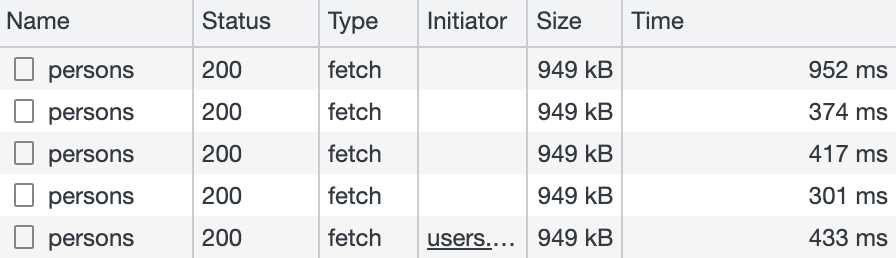
\includegraphics[scale=0.7]{img/sans-redis.png}
    \caption{Temps de réponse sans Redis}
    \label{Sans-Redis}
  \end{figure}
\subsubsubsubsection{Avec Redis}
La même requête a été réalisée mais cette fois ci avec Redis. Dans la figure 5, la première requête, sans Redis, dure une seconde, ce qui est assez conséquant. Les requêtes suivantes utilisant Redis diminuent considérablement en obtenant une moyenne de 204ms.
\begin{figure}[H]
    \centering
    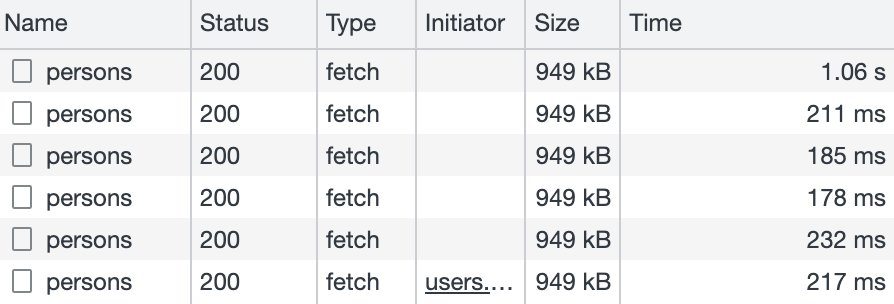
\includegraphics[scale=0.7]{img/avec-redis.png}
    \caption{Temps de réponse avec Redis}
    \label{Avec-Redis}
\end{figure}
La performance obtenue en utilisant redis a augmenté de 58,8\% ce qui justifie son utilisation.

\subsection{Caching Frontend}
Il est bien connu que les navigateurs peuvent stockées des informations relatives à la consultation de sites webs. L'application web va utiliser cette fonctionnalité à son avantage.
Plusieurs moyens de stockage existent, tels que le local storage, session storage, IndexedDB, et d'autres, tous avec leurs avantages et inconvénients. 
Àpres une analyse approfondi de ces différentes solutions, j'ai décidé d'opter l'IndexedDB. 
\subsubsection{IndexedDB}
L'IndexedDB est un système de base de données qui permet de sauvegarder des informations de manière structurée dans le navigateur. Par exemple, lorsqu'il y a une quantité importante d'informations qu'il faut aller rechercher, comme des matériaux, ces données peuvent être stockées à cet endroit ci.
\newpage
\subsubsection{Implémentation}
La récupération de données depuis l'API ne se fait plus systèmatiquement. L'application web va appliqué la logique expliquée dans la figure suivante.
\begin{figure}[H]
  \centering
  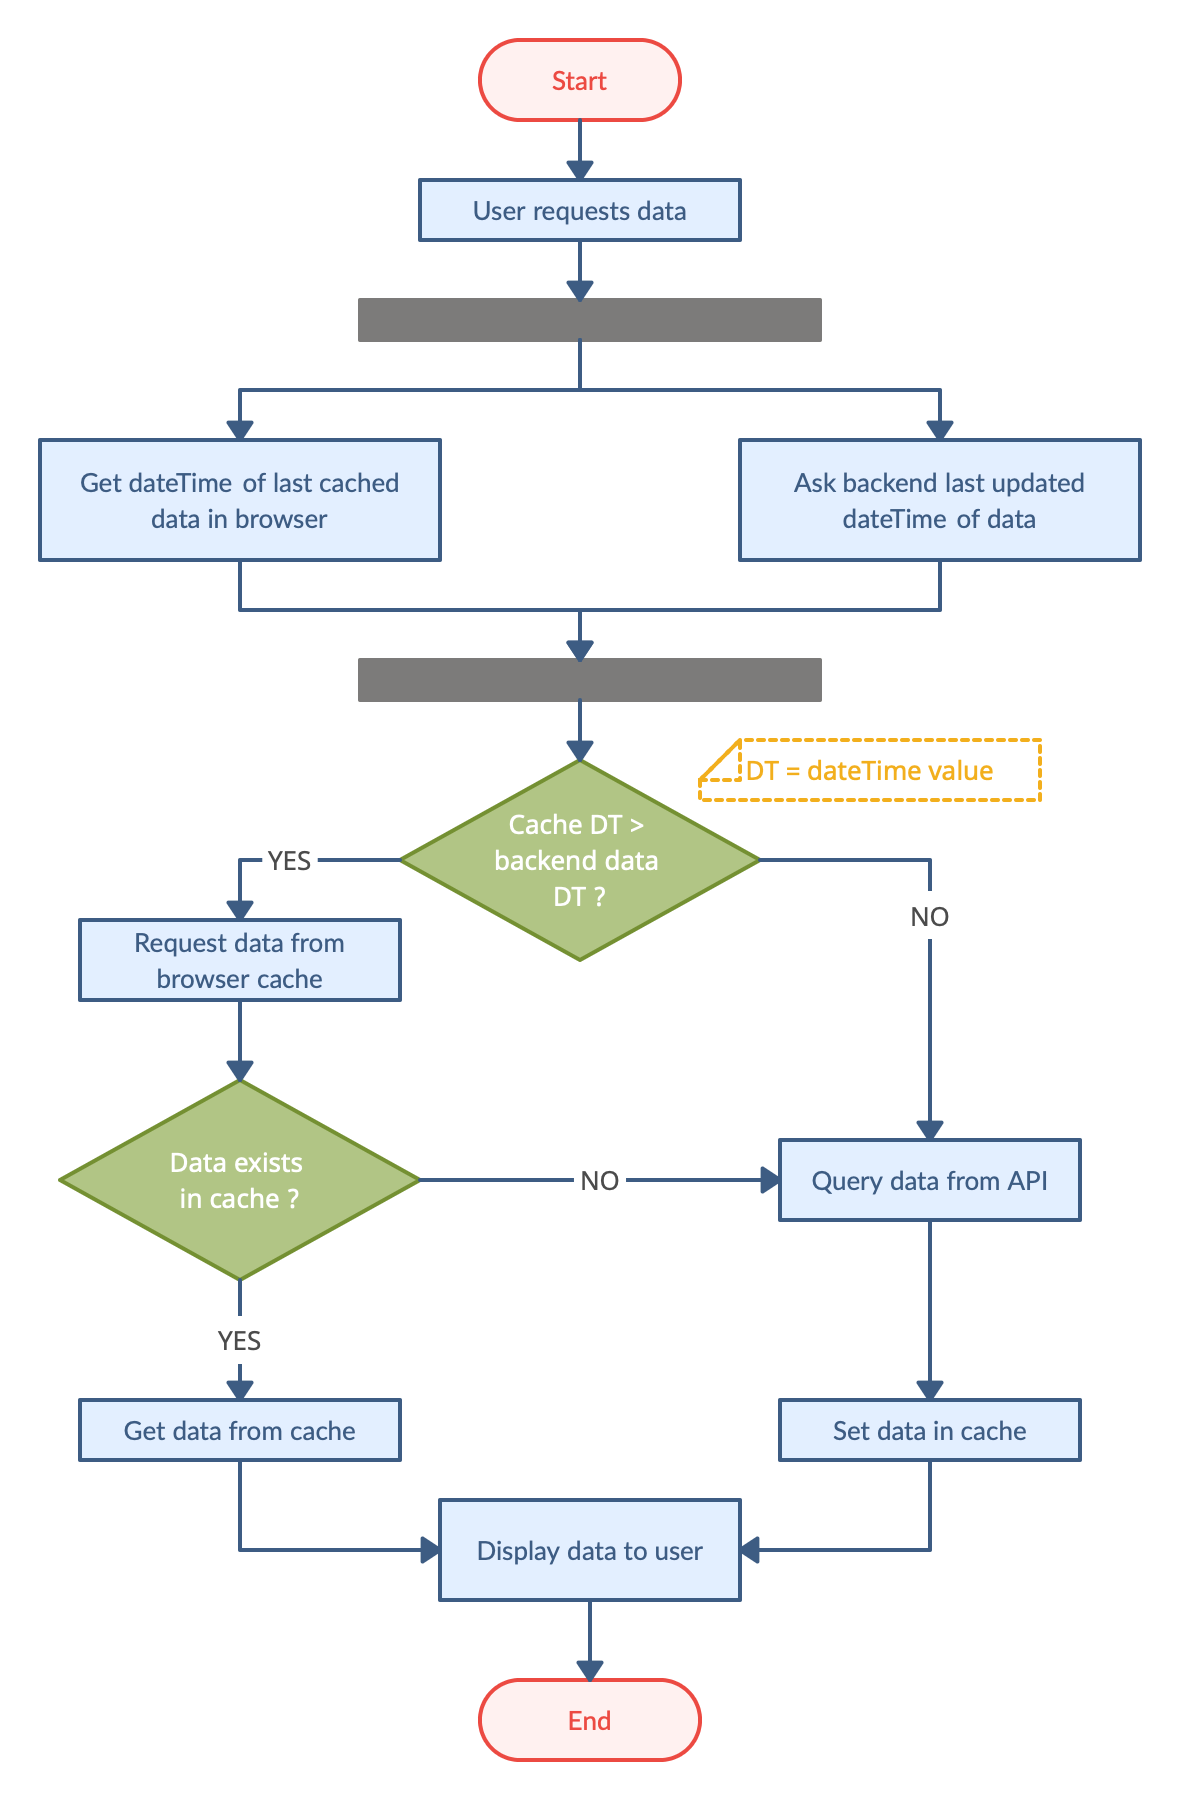
\includegraphics[scale=0.3]{img/flowchartFrontend.png}
  \caption{Flux de récupération de données}
  \label{Flux de recuperation}
\end{figure}
Cette technique permet de réduire considérablement le temps d'accès aux données de l'application.
\subsubsection{Difficultés rencontrées}
Initialement, le backend renvoyait uniquement un status indiquant si les données d'une certaine table avaient été modifiées préalablement ou non. 
Ce status était remis à l'état initial (c.à.d. "non modifiée") au moment d'une requête de type GET. Étant donnée qu'au frontend, après modification d'une donnée, l'ensemble des données mise à jours sont récupérees du backend, uniquement la personne ayant modifiée les données se verra recevoir le status "modifiée".

Les autres utilisateurs de l'application ne recevaient dès lors jamais les modifications.

Pour palier à ce problème, le backend renvoie dès à present la dérniere date de modification des données de la table. 
Le frontend compare ensuite cette date à la date de création du cache pour ces données là et si la date de création du cache est inférieure à la dernière date de mise à jour de données, il ira rechercher les données au backend.